%%%%%%%%%%%%%%%%%%%%%%%%%%%%%%%%%%%%%%%%%%%%%%%%%%%%%%%%%%%%%%%%%%%%%%%%%%%%%%%
% Definici�n del tipo de documento.                                           %
% Posibles tipos de papel: a4paper, letterpaper, legalpapper                  %
% Posibles tama�os de letra: 10pt, 11pt, 12pt                                 %
% Posibles clases de documentos: article, report, book, slides                %
%%%%%%%%%%%%%%%%%%%%%%%%%%%%%%%%%%%%%%%%%%%%%%%%%%%%%%%%%%%%%%%%%%%%%%%%%%%%%%%
\documentclass[11pt, spanish, a4paper]{article}

%%%%%%%%%%%%%%%%%%%%%%%%%%%%%%%%%%%%%%%%%%%%%%%%%%%%%%%%%%%%%%%%%%%%%%%%%%%%%%%
% Los paquetes permiten ampliar las capacidades de LaTeX.                     %
%%%%%%%%%%%%%%%%%%%%%%%%%%%%%%%%%%%%%%%%%%%%%%%%%%%%%%%%%%%%%%%%%%%%%%%%%%%%%%%
\usepackage[spanish]{babel}     % Paquete para definir el idioma usado.
\usepackage[latin1]{inputenc}   % Define la codificaci�n de caracteres 
                                % (latin1 es ISO 8859-1)
%\usepackage[T1]{fontenc}        % Agrega caracteres extendidos al font
\usepackage{t1enc}
\usepackage{palatino}           % Cambia el font por omision a Palatino
\usepackage{graphicx}           % Paquete para inclusi�n de gr�ficos.
%%%%%%%%%%%%%%%%%%%%%%%%%%%%%%%%%%%%%%%%%%%%%%%%%%%%%%%%%%%%%%%%%%%%%%%%%%%%%%%

% T�tulo principal del documento.
\title{\textbf{The Speaker (Trabajo Pr�ctico Nro. 1)}}

% Informaci�n sobre los autores.
\author{    
            Juan Manuel Barrenche, \textit{Padr�n Nro. 86.152}               \\
            \texttt{ snipperme@gmail.com }                                   \\
            Mart�n Fern�ndez, \textit{Padr�n Nro. 88.171}                    \\
            \texttt{ tinchof@gmail.com }                                     \\
            R�l Lopez, \textit{Padr�n Nro. 88.430}                           \\
            \texttt{ rau\_carpo@hotmail.com }                                \\
            Marcos J. Medrano, \textit{Padr�n Nro. 86.729}                   \\
            \texttt{ marcosmedrano0@gmail.com }                              \\
            Federico Valido, \textit{Padr�n Nro. 82.490}                     \\
            \texttt{ fvalido@gmail.com }                                     \\ 
                                                                             \\
            \normalsize{Grupo Nro. 11 (YES) - 1er. Cuatrimestre de 2009}     \\
            \normalsize{75.06 Organizaci�n de Datos}                         \\
            \normalsize{Facultad de Ingenier�a, Universidad de Buenos Aires} \\
       }
\date{DIA de MES de 2009}


% define que archivos seran realmente incluidos
%\includeonly{intro,arch,file,buffer,serializer,persistence}

% Comienzo del documento
\begin{document}

\maketitle                % Inserta el t�tulo.
%\thispagestyle{empty}     % Quita el n�mero en la primer p�gina.

% Resumen que aparece en la primera p�gina (antes de la tabla de contenidos)
\begin{abstract}
Este parrafo deber�a contener una breve descripci�n del trabajo practico. No 
deber�a contener mas de 100 palabras.
En una introducci�n posterior se podr� describir con m�s detalle los contenidos
de este trabajo.
Documento desarrollado en LATEX.
\end{abstract}

\tableofcontents        % Comentar si no se desea la Table Of Content.


% Inclusi�n de archivos externos
\input{a}
%\include{intro}         % Introducci�n
%\section{Arquitectura}

El Main ser� simplemente una vista de WordService que es el backend de la aplicaci�n y quien brinda todos los servicios a la vista. Estos servicios son:
\begin{enumerate}
\item Agregar un Documento.
\item Realizar una b�squeda.
\item Reproducir un Documento.
\end{enumerate}

Veamos la arquitectura parte por parte. Pero antes definamos el concepto de Documento, que es com�n a todas las partes.

\subsection{Documento}

Es una interfaz que permite manejar un documento obteniendo de �l renglones.
Posee tres implementaciones, una que contiene un documento totalmente en memoria, otra que trabaja con un archivo que lee desde disco a medida que va necesit�ndolo, y otra que trabaja con los documentos prealmacenados que obtiene de forma \textit{lazy}.

Ahora si, veamos la arquitectura de cada una de las partes antes mencionadas.

\subsection{Agregar un Documento}

Se divide en divide en dos grandes partes:
\begin{enumerate}
\item Agregarlo al indice.
\item Agregarlo al diccionario de sonidos.
\end{enumerate}

Existe una caracter�stica en com�n entre estas dos partes: el parseo. Es por eso que la arquitectura se defini� de tal forma que el parseo se haga en una sola oportunidad como se mostrar� luego (esto tiene una peque�a consecuencia que se mencionar� al explicar la adici�n al diccionario de sonidos).

\subsubsection{Agregar un Documento al indice}


Quien se encarga de realizar esto es el \textit{Crawler}, quien recibir� un \textit{Documento}. En primer lugar le pasa el documento al \textit{Parser} que lo utilizar� como fuente para datos.

El Parser permite manejar un documento en forma de \textit{Frases}, entendiendo por tal a un conjunto de palabras separadas por un signo de puntuaci�n (\textit{'.', ',', ';', '?', '!'}, etc.). A estas frases les aplicar� un reemplazo de s�mbolos diacr�ticos, retiro de s�mbolos extra�os, s�mbolos num�ricos, etc, y case folding, obteniendo por resultado una lista de palabras limpia. De esta manera el \textit{Crawler} puede obtener \textit{Frases} limpias desde el parser al que inicialmente le pasa el documento como fuente.

La colecci�n de palabras obtenida ser� procesada por el m�dulo \textit{StopWords Discriminator}, cuya implementaci�n tendr� un listado en memoria (que levanta al iniciar la aplicaci�n desde un archivo) de frases y de palabras sueltas que son stop words para hacer el procesamiento.

El \textit{Crawler} obtiene del \textit{StopWords Discriminator} una colecci�n (ordenada o desordenada, no importa, pero con repeticiones, si importa) de palabras que no contienen stop words. Esta colecci�n (correspondiente a una sola \textit{Frase}) le ser� entregada al \textit{Indexer}.

El \textit{Indexer} es la interfaz utilizada para acceder al �ndice (un \textit{�rbol b\#}) (tambi�n podr�a haberselo llamado Index en vez de Indexer). El \textit{Crawler} maneja una session con el \textit{Indexer}, que comienza al procesar un \textit{Documento} y termina al agregar la �ltima \textit{Frase} (cuando el \textit{Parser} deja de brindarle datos). El \textit{Indexer} parametriza un \textit{BTree\#}, un m�dulo que maneja un �rbol b\# de manera gen�rica. El \textit{Indexer} a su vez maneja una session id�ntica a la que tiene con el \textit{Crawler} con el m�dulo \textit{Inversion Sort Handler}, y solo agregar� las palabras al �rbol una vez que el \textit{Crawler} finalice la session con el \textit{Indexer}.

El \textit{BTree\#} es una implementaci�n gen�rica de �rbol b\# que utiliza 2 archivos, uno para nodos internos y otro para hojas, y que maneja una equiparaci�n entre nodos y bloques. Utiliza el \textit{VariableLengthFileManager} en su implementaci�n en disco. Debe ser parametrizado con una \textit{Key} (clave de los nodos internos) y un \textit{Element} (registro de las hojas que contiene entre otras cosas a la clave). Este \textit{Element} se definir� de tal manera que tenga el listado de \textit{Documentos} en su interior; este listado de \textit{Documentos} se implementar� utilizado el \textit{VariableLengthFileManager}. No se muestra a \textit{Key} ni a \textit{Element}, ni al archivo del listado de \textit{Documentos} en el diagrama por simplificaci�n. Adem�s deben brindarse los \textit{Serializer} correspondientes a una colecci�n ordenada de \textit{Keys} y de \textit{Elements} para parametrizar al \textit{BTree\#}.

Las sessiones mencionadas (entre el \textit{Crawler} y \textit{Indexer}, y entre el \textit{Indexer} y el \textit{Inversion Sort Handler}) sirven para evitar tener un documento completo en memoria.

Al mismo tiempo que el \textit{Crawler} va procesando las frases, va a agregando todas las palabras encontradas en un Set (conjunto sin repeticiones), de esta manera obtiene el vocabulario completo. Ese Set ser� devuelto al \textit{WordService} como respuesta al pedido de indexar un documento.

\subsubsection{Agregar un Documento al diccionario de sonidos}

Como puede adivinarse, el vocabulario completo obtenido al agregar un docuemento al �ndice es la entrada usada para realizar el agregado al diccionario de sonidos. Esto tiene como consecuencia que el agregado de sonidos ser� en distinto orden al original del documento. Pero tiene como ventaja el no tener que procesar dos veces el documento por el \textit{Parser} (y a no tener que leerlo de nuevo desde disco si es que no se lo quiere tener completo en memoria como planteamos antes).

El m�dulo usado para esta acci�n es el llamado \textit{WordsRecorder}.

Si bien se modific� levemente la interacci�n entre los m�dulos, la arquitectura es b�sicamente la misma que para la entrega 1, y la interacci�n entre m�dulos puede verse claramente en el esquema.

La �nica gran modificaci�n consiste en el reemplazo del "�ndice secuencial de sonidos" por un \textit{Trie}, que utiliza para su implementaci�n un \textit{VariableLengthFileManager}.

\subsection{Realizar una B�squeda}

Esta acci�n es responsabilidad del \textit{Search Engine}. Para hacerlo primero debe limpiar la cadena de b�squeda, para lo cual interactura con el \textit{Parser} y con el \textit{StopWords Discriminator}.
Una vez que tiene la consulta limpia, realiza la b�squeda utilizando el \textit{Indexer}, que a su vez utilizar� el \textit{BTree\#}.

El \textit{SearchEngine} realiza las operaciones de ordenado necesarias y devuelve un listado ordenado de \textit{documentos}.

\subsection{Reproducir un Documento}

La reproducci�n la realizar� el \textit{DocumentPlayer}, que recibir� un \textit{Documento} que deber� parsear utilizando el \textit{Parser}. A medida que va obteniendo las palabras correspondientes las ir� reproduciendo delegando toda la complejidad en el \textit{WordsPlayer}.

El \textit{WordsPlayer} es la contrapartida del \textit{WordsRecorder} explicado antes, y su arquitectura es coincidente con la de este.

\subsection{VariableLengtFileManager - Archivo de registros de longitud variable en bloques}
El \textit{VariableLengthFileManager} que ya exist�a en la entrega anterior, ahora permite actualizaciones de los registros.
Recordemos que el \textit{Address} en este archivo consta de dos partes. La primera el bloque donde se encuentra el registro y la segunda el n�mero de objeto que representa el registro. Ahora bien, si una actualizaci�n de un registro aumentara el tama�o del mismo y esto hiciera que la suma de los tama�os de los registros que se encuentran en dicho bloque excediera el tama�o del bloque hay que hacer una reestructuraci�n de los datos. Existen varias alternativas para ello:
\begin{enumerate}
\item Tomar como pol�tica de reestructuraci�n la decisi�n de s�lo mover los objetos del final que excedan a la capacidad del bloque. Este es, para nuestro caso, impracticable ya que implicar�a actualizar todos los datos que tuvieran referencias a dichos objetos. 
\item Quitar �nicamente al objeto que se est� actualizando en dicho momento. Esto pareciera traer el mismo inconveniente, ya que al hacer esto, las direcciones de los subsiguientes registros tambi�n se ver�an modificadas porque en el bloque existe un objeto menos y el conteo quedar�a diferido en uno (es decir, que si quit� el registro cuyo n�mero de objeto 2 el siguiente, con n�mero de objeto 3, pasar�a a ser el objeto numero 2). 
\end{enumerate}
Entonces, para aplicar la segunda opci�n se debe evitar que los objetos siguientes al modificado mantengan su lugar en la lista. As� fue que se introdujo el concepto de \textbf{nullObject}.

\subsubsection{NullObject}
El \textbf{nullObject} es el encargado de ocupar el lugar que originalmente ocupaba un objeto que se encontraba compartiendo un bloque con otros registros y que, luego de su actualizaci�n, provoc� un desborde del bloque.
Ahora bien, recordemos que los objetos se encuentran serializados, y que la manera de rehidratandos es para todos la misma. Por lo cual necesitamos que los serializadores puedan hidratar \textbf{nullObject} sin intervenci�n de un proceso de verificaci�n, ni tener que estar agregando metadata listando los objetos que fueron retirados del bloque. Para ello se extendi� la interfaz \textit{Serializer} a una nueva llamada \textit{NullableSerializer} la cual indica que dicho serializador puede serializar e hidratar \textbf{nullObjects}. 
Todas nuestras implementaciones del NullObject se corresponden al valor \textbf{null} de Java, pero no tiene por qu� ser as�. El requisito es que el m�todo \textit{NullableSerializer\#dehydriateNull} modifique el Buffer de salida con, a lo sumo, el m�nimo tama�o de serializaci�n de los objetos no nulos y que adem�s, claro est�, el \textit{NullableSerializer\#hydrate} pueda interpretar esa informaci�n como un objeto mas (o la referencia \textbf{null}). Este requisito de m�ximo tama�o para la serializaci�n del \textbf{nullObject} se debe a que este objeto debe terminar ocupando menos que el objeto que lo que ocupaba el objeto a reemplazar antes de intentar ser modificado por el nuevo objeto. De esta manera, sabemos que, al quitarlo, los registros restantes y el \textbf{nullObject} van a caber en el bloque.

\subsubsection{Resultado final}
Finalmente las actualizaciones quedan de la siguiente manera y se distinguen tres casos de \textbf{desborde}:
\begin{enumerate}
\item Actualizaci�n de un registro que se encuentra solo en un bloque
\item Actualizaci�n de un registro que se encuentra como �ltimo registro del bloque
\item Actualizaci�n de un registro que no se encuentra como �ltimo registro del bloque
\end{enumerate}

\paragraph{Actualizaci�n de un registro que se encuentra solo en un bloque}

Este caso es el mas sencillo, ya que el registro est� solo y puede extenderse a m�ltiples bloques. Esto est� solucionado en los \textit{writers}, que agregar�n la metadata necesaria para asociar los bloques como si fueran uno solo. De manera que los \textit{readers} puedan leer toda la informaci�n en conjunto. \footnote{En este caso la direcci�n del objeto NUNCA cambia}

\paragraph{Actualizaci�n de un registro que se encuentra como �ltimo registro del bloque}

Este caso es el que le sigue en simplicidad. No requiere tampoco la intervenci�n de los \textbf{nullObjects}, solamente se retira el objeto del bloque y se lo hace ingresar nuevamente al archivo como una inserci�n. Esto nos devuelve una direcci�n que es la que se retorna como resultado de la actualizaci�n del registro para que el que solicit� la actualizaci�n modifique las referencias que pose�a hacia el registro.

\paragraph{Actualizaci�n de un registro que no se encuentra como �ltimo registro del bloque}

Al igual que en el caso anterior, se retira el objeto que se est� actualizando, pero esta vez se lo reemplaza por un \textbf{nullObject}. Nuevamente se procede al agregado del objeto al archivo por medio de una inserci�n que nos devolver� la nueva direcci�n del objeto que ser� enviada al que solicit� la actualizaci�n para que pueda actualizar todas las referencias que posee al objeto. Vemos que gracias a este concepto (\textbf{nullObject}) los casos quedaron todos similares y sin gran complejidad.

\paragraph{An�lisis de ventajas y desventajas}

Esta soluci�n permite que, a lo sumo, un �nico registro modifique su direcci�n y que dicho registro sea el que se solicit� actualizar, lo que nos garantiza que es un dato con el que se est� trabajando y que su \textit{Address} puede ser modificado donde sea pertinente. 

La desventaja que parece tener es que los bloques se empiezan a llenar con datos que no nos interesa almacenar (los \textbf{nullObjects}). Para evitar esto se pueden implementar pol�ticas de reorganizaci�n de bloques. �C�mo ser�a esto? Bueno, a simple vista se puede observar que si tengo que retirar el registro que se encuentra en la �ltima posicisi�n del bloque todos los nullObjects anteriores (hasta encontrar un objeto que no lo sea) pueden ser tambi�n retirados del bloque, ganando, de esta manera, mas espacio para los otros registros que se encuentran en el bloque y que ser� utilizado cuando dichos registros necesiten expandirse. Finalmente, cuando se actualice el �ltimo de los registros reales restantes en el bloque (es decir, el registro que se encuentra en un bloque donde, excluy�ndolo a �l mismo, en el bloque solo hay \textbf{nullObjects}) este puede retirar todas esas referencias a nullObjects quedando como �nico propietario del bloque. \footnote{Si bien estas pol�ticas no se encuentran implementadas, debido a falta de tiempo, son facilmente implementables y otorgan un mayor aprovechamiento del espacio reduciendo la fragmentaci�n interna}

\subsection{StraightVariableLengthFile - Archivo de registros de longitud variable sin bloques}

Se agreg� una forma mas de persistencia en archivos \textit{StraightVariableLengthFile}. Esta implementaci�n de archivo basa su funcionamiento en los mismos lineamientos que el \textit{VariableLengthFileManager} en la primera parte, exceptuando que no trabaja por bloques. Por lo cual cada registro es serializado a continuaci�n del �ltimo. Para recuperar un registro ya almacenado se recibe el \textit{Address} (que en este caso corresponde �nicamente a un Offset y que fue entregado por el \textit{StraightVariableLengthFile} al momento de agregarse dicho registro) y se utiliza el Serializador con que fue configurado para hidratar el registro que luego es devuelto al usuario. Las ventajas de esta implementaci�n, respecto a la de por bloques, es que los archivos quedan mas densos y no requiere meta data dentro del archivo (mas all� de la que requiera la serializaci�n, la cual es independiente de la implementaci�n del archivo).

Qued� pendiente, como idea, permitirle al usuario de ambos tipos de archivos (con y sin bloques) que posea una secci�n con datos reservados (al estilo meta-data) que puedan serializarse de manera diferente que el com�n de los registros. Observamos que esto ser�a �til en numerosos casos. Como simples ejemplos, si quisiera almacenar la cantidad de registros en el l�xico, si quisiera guardar en �rbol el nombre para el archivo de hojas, etc. Si bien, nuestros casos los resolvimos implementando serializadores con estado a los que se le indicaba que tipo de dato esperaban recibir, entendemos que esta configuraci�n complica algo que en concepto es mas sencillo.

\subsection{Otros datos relevantes de la arquitectura}

Se incorpor� la abstracci�n \textit{StraightVariableLengthFile} para el archivo de sonidos (que antes era un \textit{VariableLengthFileManager}) por lo que ahora el archivo correspondiente es 100\% denso. 

El \textit{VariableLengthFileManager} posee dos implementaciones, una que maneja cach� de bloques y la otra que no. La primera se usa en casos como el trie ya que todos los registros poseen un mismo serializador (recordemos que el trie est� implementado en dos archivos) y la segunda es utilizada en el �rbol, ya que la forma de los registros almacenados en los archivos var�a durante la vida del �rbol y esto fuerza al uso de un serializador mas dependiente del �rbol y esto complica el manejo del cach�.

\begin{figure}[!htp]
\centering
\makebox[\textwidth]{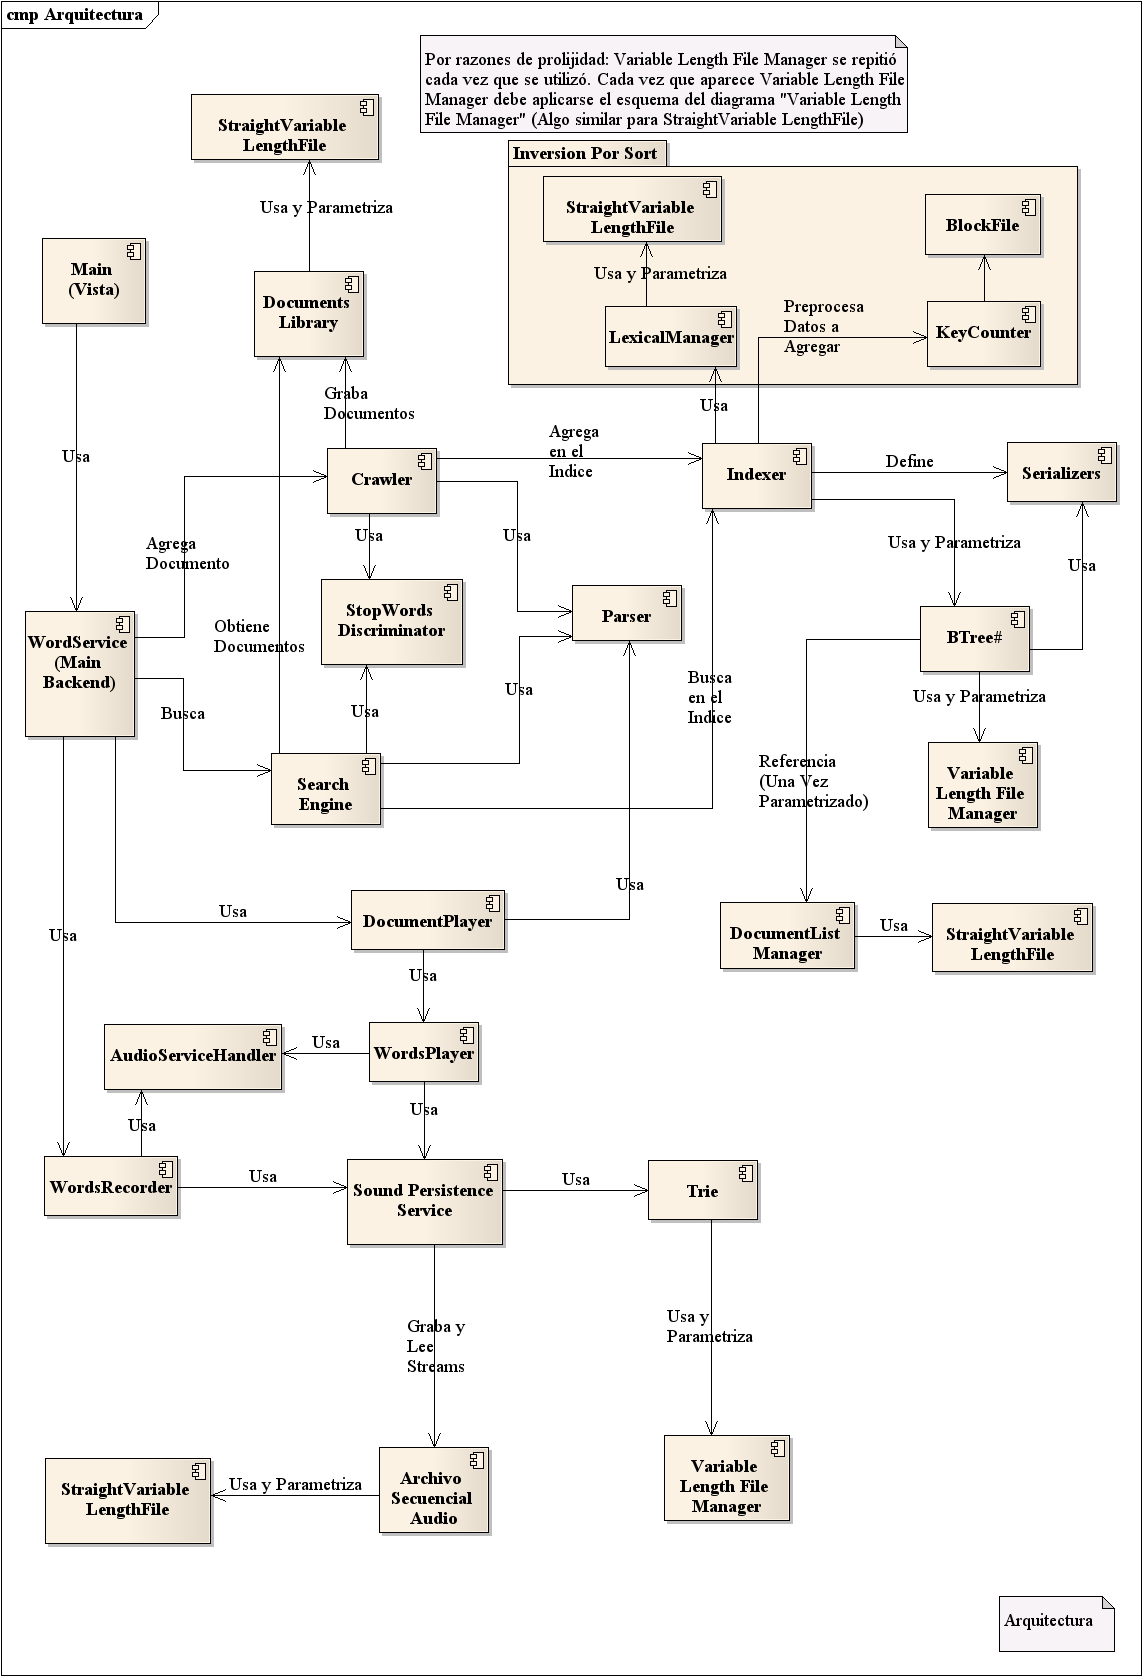
\includegraphics[scale=0.4,natwidth=20pt,natheight=10pt]{img/Arch2daEntrega.png}}
\caption{Arquitectura VariableLengthFileManager} 
\end{figure}

\begin{figure}[!htp]
\centering
\makebox[\textwidth]{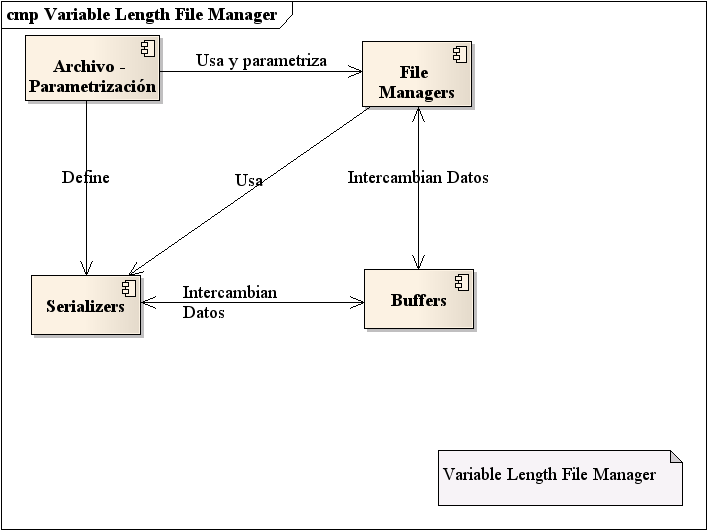
\includegraphics[scale=0.5,natwidth=20pt,natheight=10pt]{img/VariableLengthFileManager.png}}
\caption{Arquitectura VariableLengthFileManager}
\end{figure}

\begin{figure}[!htp]
\centering
\makebox[\textwidth]{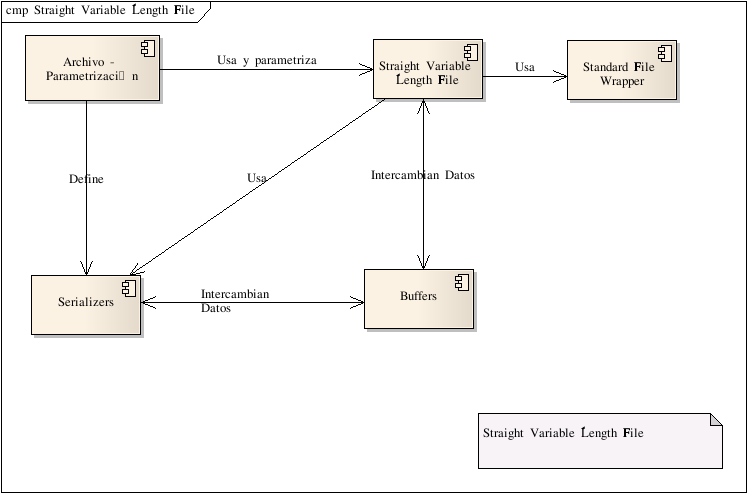
\includegraphics[scale=0.5,natwidth=20pt,natheight=10pt]{img/StraightVariableLengthFile.png}}
\caption{Arquitectura StraightVariableLengthFile}
\end{figure}

          % Descripci�n general de la Arquitectura e introducci�n de cada Modulo
%\include{file}          % Manejadores de Archivos
%\include{buffer}        % Buffers de Entrada y Salida
%\include{serializer}    % Serializadores
%\include{persistence}   % Servicios de Persistencia

\end{document}
